\documentclass[handout]{beamer}

\usepackage[frenchb]{babel}
\usepackage[T1]{fontenc}
\usepackage[utf8x]{inputenc}
 
\usetheme{Berkeley}
\usecolortheme{crane}
\useinnertheme{rounded}

\title[Saint-Venant]{Présentation projet : les équations de Saint-Venant et la méthode des éléments finis}
\author{Gabrielle \bsc{Collette}, Conrad \bsc{Hillairet} \& Alexandre \bsc{Vieira}}
\institute{INSA de Rouen}
\date{30 mai 2014}


\AtBeginSection[]
{
	\begin{frame}
		\frametitle{Sommaire}
		\tableofcontents[currentsection, hideothersubsections]
	\end{frame}
}

\begin{document}

\begin{frame}
\titlepage
\end{frame}

\begin{frame}
	\frametitle{Sommaire}
	\tableofcontents
\end{frame}

\section{Les équations de Saint-Venant}
\subsection[Hydrodynam.]{Un peu d'hydrodynamique} %Exemples
 
\begin{frame}
	\frametitle{Cas d'utilisation des équations de Saint-Venant}
		Valables lorsque la hauteur du liquide est négligeable par rapport à sa largeur. Exemple : une baignoire\\
		Utilisées en météorologie, modélisation des océans. 
\end{frame}

\subsection[Équations]{Présentation des équations}

\begin{frame}
	\frametitle{Démonstration : grandes idées}
	%Partir sur un raisonnement par intégrale, avec un volume quelconque. Mais vu que c'est quelconque, on arrive à ça !
	\[\hspace{-10em}\left.\begin{array}{c} \text{Équation de continuité} \\ \text{Équation de quantité de mouvement} \end{array}\right\}\] 
	\[\hspace{10em}\Rightarrow \text{Équations de Navier-Stokes} \]
	\[\left\{ \begin{array}{c c c}
	\frac{\partial \rho}{\partial t} + div\left(\rho \overrightarrow{U}\right)&=&0\\
	\frac{\partial}{\partial t} \left( \rho \overrightarrow{U} \right) + div\left( \rho \overrightarrow{U} \otimes \overrightarrow{U}\right) &=& \rho f -\nabla p + div(\tau)
\end{array}\right.\]
	%Donner définition de chaque notation
\end{frame}

\begin{frame}
	\frametitle{Équations de Saint-Venant complètes}
	%Différentes hypothèses : Boussinesq, pression hydrostatique, vitesse moyenne
	\begin{itemize}
		\item Moyenne des équations sur la hauteur, eau peu profonde.
		\item Transformation des équations de Navier-Stokes
	\end{itemize}

	\[	\left\{ \begin{array}{c c c}
	\frac{\partial}{\partial x} (hu) + \frac{\partial}{\partial y} (hv) + \frac{\partial h}{\partial t} &=& 0 \\
      \frac{\partial u}{\partial t} + u\frac{\partial u}{\partial x} + v\frac{\partial u}{\partial y} &=& -g\frac{\partial Z_s}{\partial x} + F_x\\
	 \frac{\partial v}{\partial t} + u\frac{\partial v}{\partial x} + v\frac{\partial v}{\partial y}&=& -g\frac{\partial Z_s}{\partial y} + F_y
	\end{array}\right.	\]
\end{frame}

\begin{frame}
	\frametitle{Équations de Saint-Venant linéarisées}
	Hypothèses encore plus simplificatrices (variation d'hauteur et de vitesse faibles)
	\[	\left\{ 
	\begin{array}{c c c}
		\frac{\partial u}{\partial t}	& = & -g \frac{\partial \eta}{\partial x}\\
		\frac{\partial v}{\partial t} & = & -g  \frac{\partial \eta}{\partial y}\\
      \frac{\partial \eta}{\partial t} & = & - h_0  (\frac{\partial u}{\partial x}+\frac{\partial v}{\partial y} )\\
		
		
	\end{array}
	\right.\]
\end{frame}

\section{Méthode des éléments finis}
\subsection[Présentation]{Présentation rapide de la méthode}
\begin{frame}
	\frametitle{Equation de départ}
	On part de l'équation suivante :\\
	$\left\{\begin{matrix}
		-\Delta\left(u\right)=f, u\in\Omega\\
		u=0 \textit{ sur } \Gamma
		\end{matrix}\right.$
\end{frame}

\begin{frame}
	\frametitle{Théorème de Lax-Milgram}
	On transforme ce problème en : trouver u solution de \\
	$a\left(u, v\right)=L\left(v\right)$\\
	D'après le théorème de Lax-Milgram, si $a\left(.,.\right)$ est une forme bilinéaire continue et V-elliptique et si $L\left(v\right)$ est une forme linéaire continue, alors notre problème admet une solution et elle est unique.
\end{frame}

\begin{frame}
		\frametitle{Méthode des éléments finis : Définitions}
		Maillage : pavage de l'espace en volumes élémentaires. Un maillage est constituté d'une suite de points que l'on appellera noeuds\\
		Pour tout entier $k\geq 1$, on appelle treillis d'ordre $k$ l'ensemble :\\
$\Sigma_{k}=\left\{ x\in K \text{ tel que } \lambda_{j}\left(x\right)\in\left\{0, \frac{1}{k},...,\frac{k-1}{k}, 1\right\} \text{ pour }1\leq j\leq N\right\}$
$\phi_{j} $: base de $V_h$
\end{frame}

\begin{frame}
	\frametitle{Méthode des éléments finis}
	$v(x)=\sum_{i=1}^{n_{d_{l}}}v\left(\hat{a}_{i}\right)\phi_{i}\left(x\right)$\\
	Matrice de rigidité : $\mathcal{K}_{h}=\left(\int_{\Omega}\nabla\phi_{j}.\nabla\phi_{i} dx\right)_{1\leq i, j\leq n_{d_{l}}}$\\
	On obtient le système linéaire : $\mathcal{K}_{h}U_{h}=b_{h}$
	

\end{frame}
\subsection[Simulation]{Simulation sur un exemple}
\begin{frame}
	\frametitle{Formulation variationelle}
	Soit le problème suivant :
\begin{align*}
\left\{\begin{matrix}
-\Delta\left(u\right)=f,  u\in\Omega\\
u=0 \texttt{ sur }\Gamma
\end{matrix}
 \right.
\end{align*}
On a alors :
$\forall v\in V a(u,v)=L(v)$
avec\\
\begin{equation*}
a(u,v)=\int_{\Omega}\nabla u.\nabla v
\end{equation*}
\begin{equation*}
L(v)=\int_{\Omega}fv
\end{equation*}
\begin{equation*}
V=H_{0}^{1}=\left\{v\in L^{2}\left(\Omega\right), \nabla u\in L^{2}\left(\Omega\right), v=0 \texttt{ sur }\Gamma\right\}
\end{equation*}
Lax-Migram s'applique.
\end{frame}

\begin{frame}
	\frametitle{Méthode des éléments finis}
Maillage sur le carré unité avec des triangles $\mathbb{P}_{1}$. Unisolvance vérifiée.\\
équation sous la forme d'un système linéaire : $\mathcal{K}_{h}U_{h}=b_{h}$. Par exemple, si on prend $f$ égal à 0.001, on obtient :
\end{frame}

\begin{frame}
	\frametitle{Méthode des éléments finis}\begin{align*}
\mathcal{K}_{h}=\left(
\begin{matrix}
4  &    -1    &  0   &   -1    &  0  &    0   &   0  &    0  &    0\\
-1   &   4  &    -1  &    0     & -1  &    0  &    0  &    0  &    0\\
0    &  -1    &  4   &   0    &  0   &   -1 &     0   &   0 &     0\\
-1  &    0   &   0    &  4   &   -1 &     0   &   -1  &    0  &    0\\
0  &    -1   &   0   &   -1  &    4    &  -1  &    0   &   -1  &    0\\
0   &   0  &    -1   &   0   &   -1  &    4   &   0  &    0  &    -1\\
0   &   0   &   0   &   -1    &  0    &  0  &    4   &   -1   &   0\\
0    &  0    &  0   &   0    &  -1    &  0   &   -1  &    4    &  -1\\
0    &  0  &    0   &   0    &  0   &   -1   &   0    &  -1   &   4\\
\end{matrix}\right)
\end{align*}

\begin{align*}
b_h =\left(
\begin{matrix}
6.25\times 10^{-5}\\
\vdots\\
6.25\times 10^{-5}
\end{matrix}\right)
\end{align*}
Nous pouvons alors résoudre notre système.
\end{frame}

\subsection[Implém.]{Implémentation de la méthode}
\begin{frame}
	\frametitle{Bouah}

\end{frame}

\section[FreeFem++]{Saint-Venant avec FreeFem++}
\subsection[Volumes finis]{La méthode des volumes finis}
\begin{frame}
	\frametitle{Présentation de la méthode}
	%EF : pourri pour ce type d'équation. Volume fini : parfait !
	%Faire petit topo sur la méthode, avec juste un maillage. Solution constante sur un maille, tout ça tout ça.
	\centering 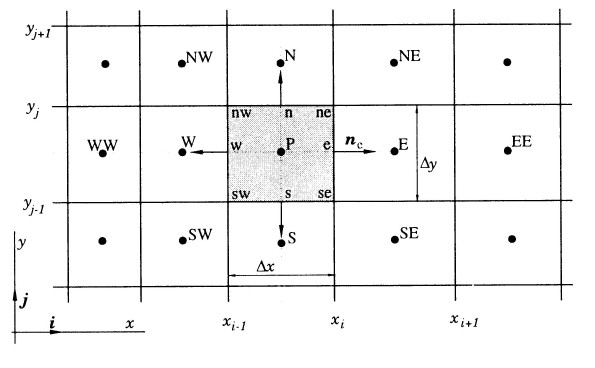
\includegraphics[scale=0.62]{3.jpg}\\
	\tiny{\underline{Source :} Cours Introduction à la Mécanique des Fluides Numériques : Méthode "Volumes Finis" - 1A HY - Alexeï Stoukov}
\end{frame}

\subsection[Simulation FF++]{Simulations avec FreeFem++}
\begin{frame}
	\frametitle{Résultats}
	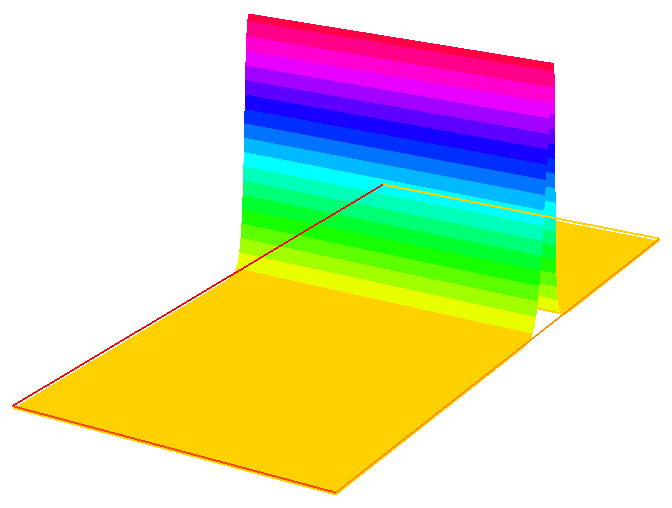
\includegraphics[scale=0.22]{../images/capture1.png}
	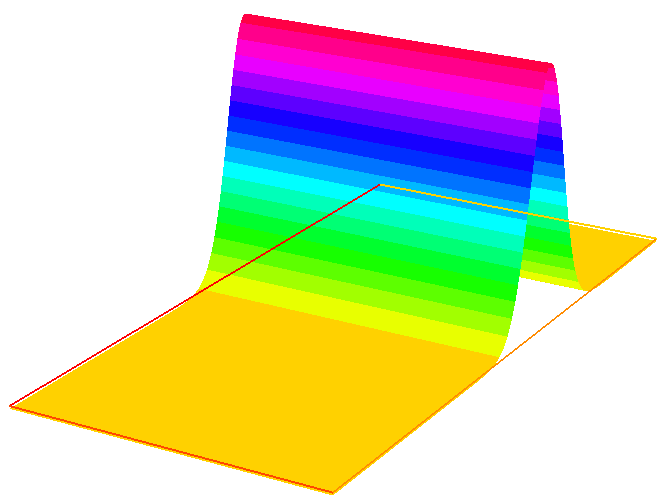
\includegraphics[scale=0.22]{../images/capture6.png}
	% Parler Sadaka, papier, etc. Essayer de faire pareil : merde encore. Parler aussi de FreeFem++
\end{frame}

\section*{Conclusion}
\begin{frame}
	\frametitle{Conclusion}
\end{frame}
\end{document}
